\documentclass[../Book.Stress_regulation.tex]{subfiles}
\graphicspath{{\subfix{../images/}}}
\begin{document}



\subsubsection{Anticipatory Coping}

\epigraph{Giving up smoking is the easiest thing in the world. I know, because I've done it thousands of times.}{\textit{Mark Twain}}

Anticipatory coping\footnote{cope, to overcome --- anticipate, is to consider an upcoming event}\index{coping!anticipatory} is efforts done {in advance} of a possible stress,  with the goal to {overcome}, reduce or tolerate the {imbalance between perceived requirements and available resources}.

Two types of coping strategies can be distinguished.

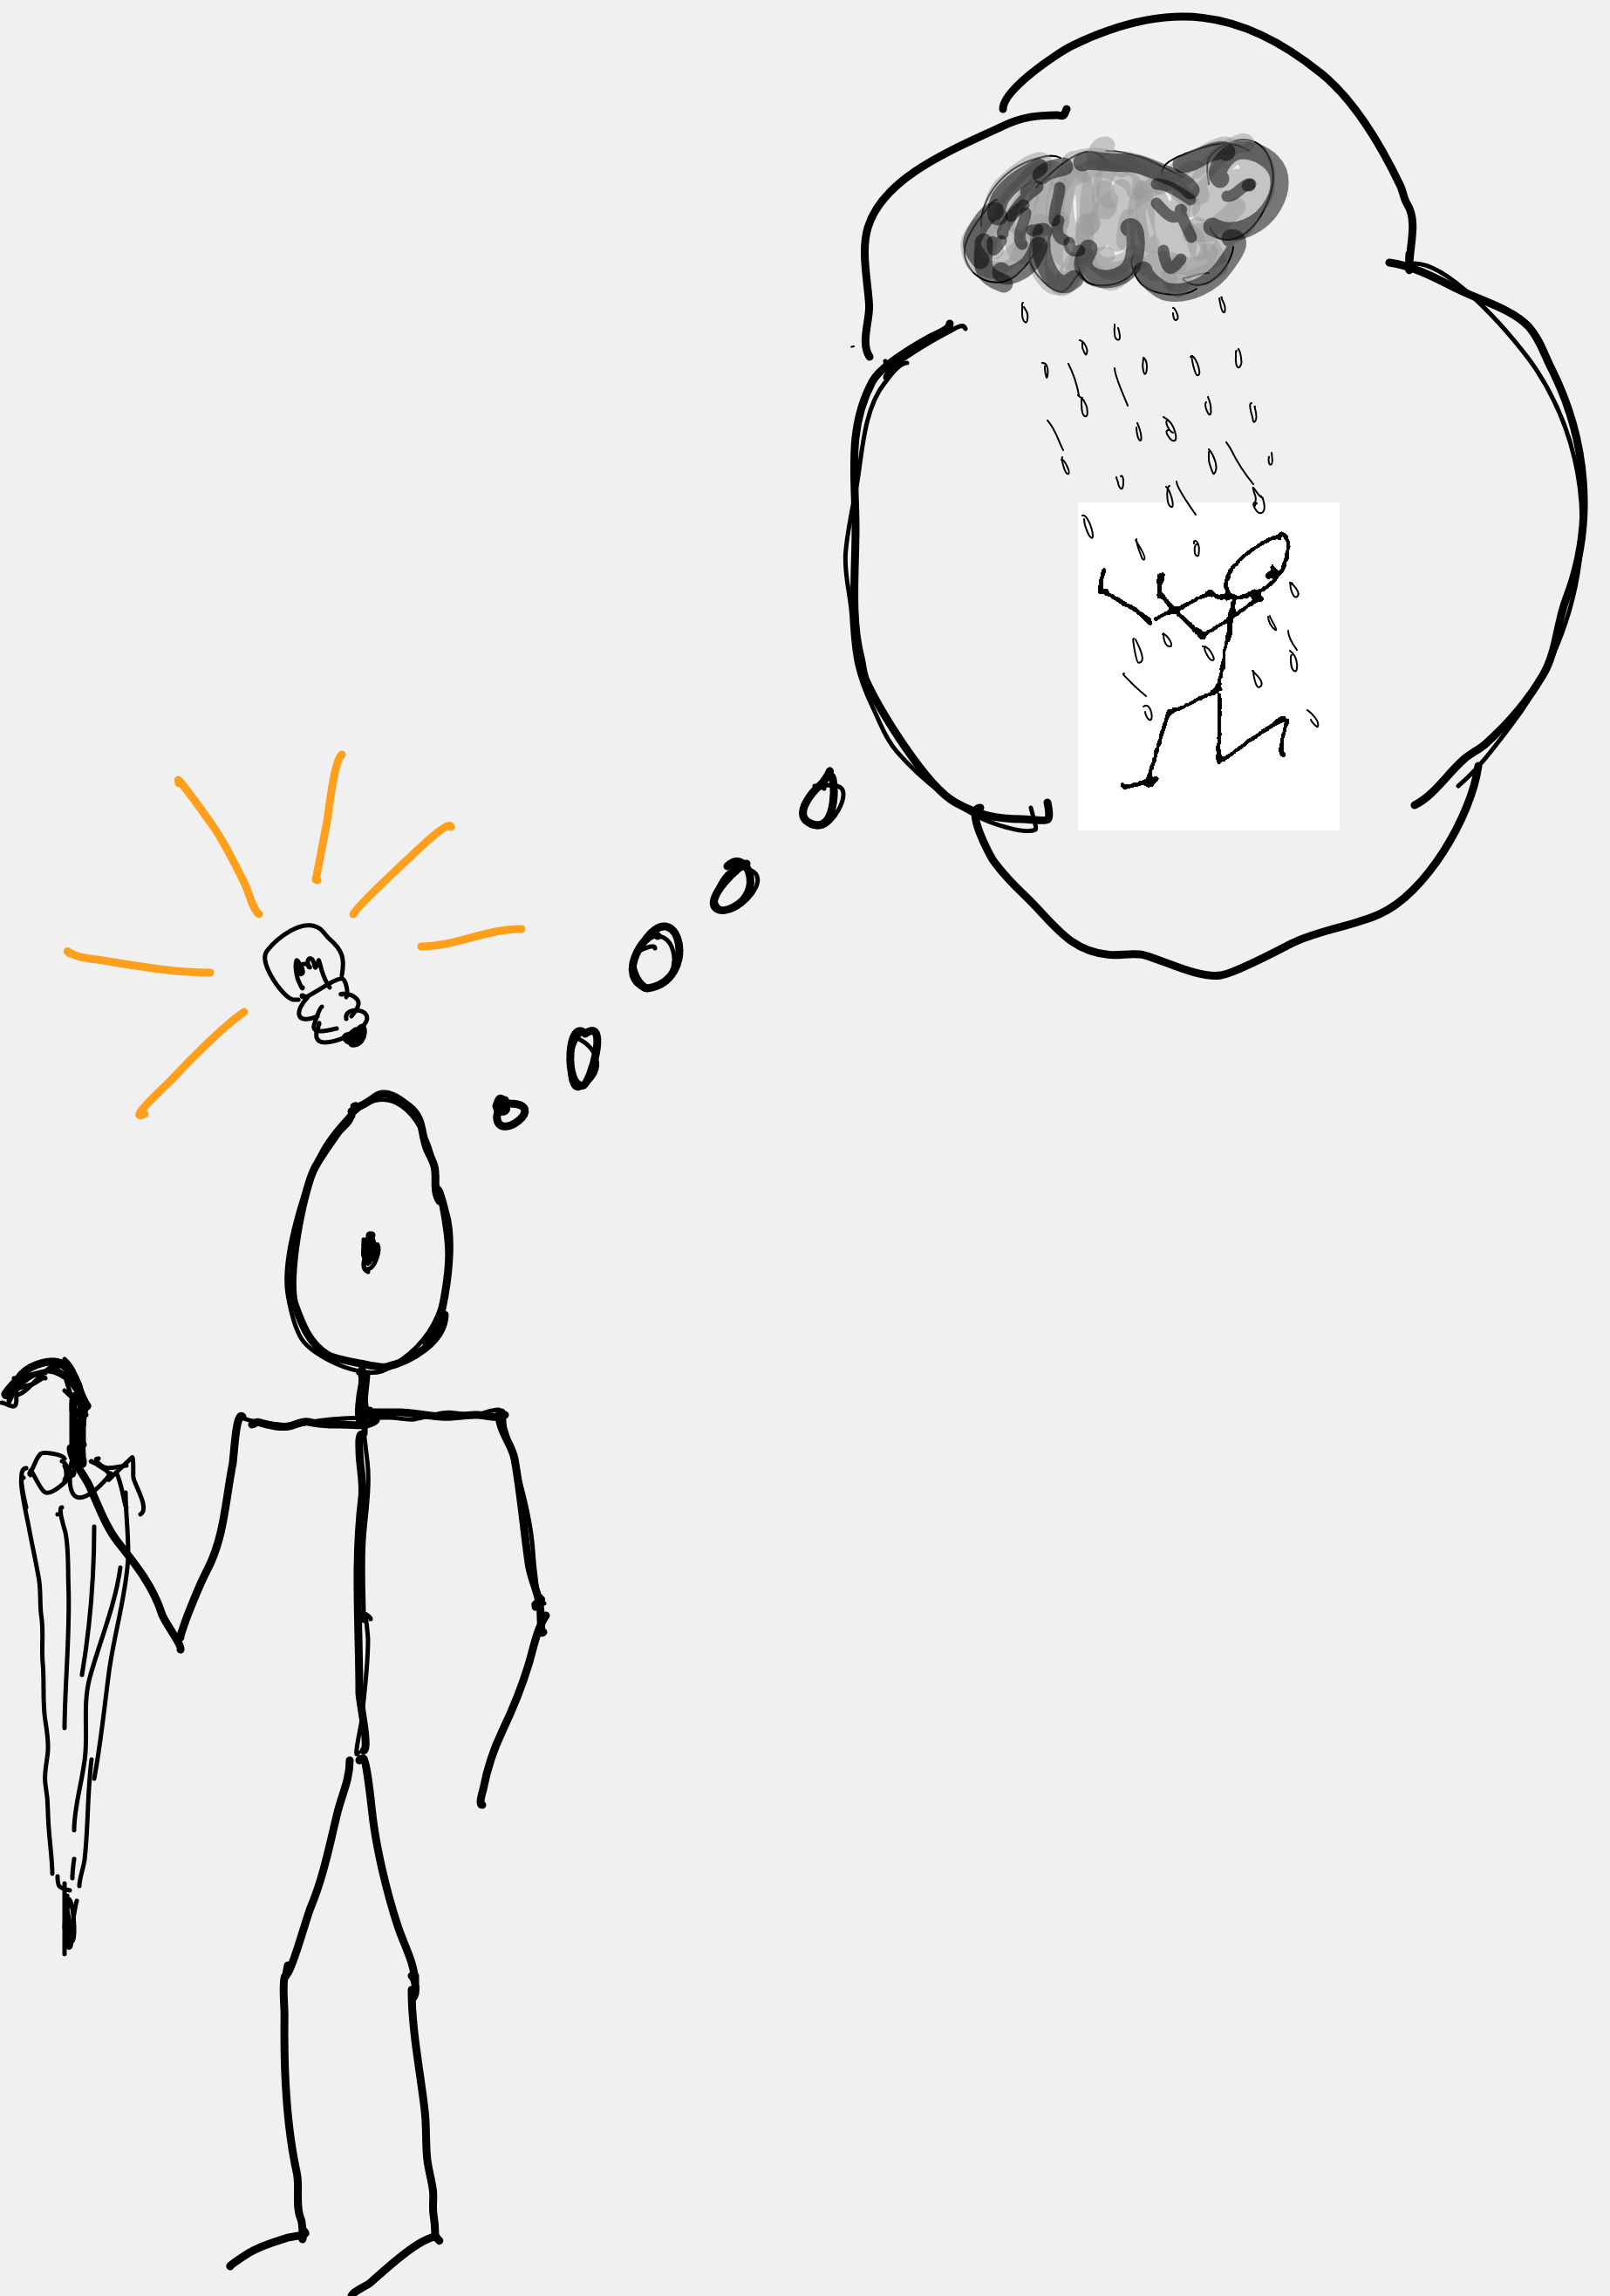
\includegraphics[width=4cm]{ACoping}

 \begin{description}
\item[Problem Oriented Coping]\index{coping!problem oriented} attempts to change the stressor or the relation to it by the means of {direct actions} and/or problem solving activities, such as to fight, in order to destroy, neutralize or weaken the threat. Flight in order to remove yourself from the threat is another possible action, or then looking for possibilities for fight or flight, like to lie, to negotiate or to make a compromise. Yet another way is to avoid future stress, by behaving in a way to increase the own tolerance or to decrease the expected future stress.
\item[Emotion Oriented Coping]\index{coping!emotion oriented} is an attempt to change yourself with activities, which make you {feel better}, without changing the stressor.
\end{description}

Some examples are relaxation and Bio feedback as Body centered activities, mind centered activities could be planning distractions, day dreaming or thinking about yourself or then therapy to regulate the conscious and subconscious mechanism which leads to additional fear.



\end{document}